%%%%%%%%%%%%%%%%%%%%%%%%%%%%%%%%%%%%%%%%%%%%%%%%%%%%%
% Gugler Labs, GNU/Linux, Trabajo Practico Final
% Segundo cuatrimestre 2017
%
% octubre 2018, rev 2
%%%%%%%%%%%%%%%%%%%%%%%%%%%%%%%%%%%%%%%%%%%%%%%%%%%%%

\documentclass[10pt,a4paper]{article}
\usepackage[utf8]{inputenc}
\usepackage[spanish]{babel}
\usepackage{siunitx}

\usepackage{hyperref}
\usepackage{booktabs}
\usepackage{placeins}
\usepackage[table,xcdraw]{xcolor}
\usepackage{epigraph}

\usepackage[framemethod=TikZ]{mdframed}
\newenvironment{unitFrame}[1][]{%
    \begin{mdframed}[%
        frametitle={#1},
        skipabove=\baselineskip plus 2pt minus 1pt,
        skipbelow=\baselineskip plus 2pt minus 1pt,
        linewidth=0.5pt,
        frametitlerule=true,
        frametitlebackgroundcolor=gray!10
    ]%
}{%
    \end{mdframed}
}

\usepackage{listings}
\lstset{
    breaklines=true,
    basicstyle=\footnotesize,
    %frame=leftline,
    texcl=true,
    basicstyle=\ttfamily,
    escapechar=!
}
\usepackage{graphicx}
\graphicspath{ {./pictos/} }

\usepackage{fancyhdr}
\setlength{\headheight}{15pt}
\pagestyle{fancy}
\lhead{}
%\chead{\includegraphics[scale=0.5]{./banner.jpg}}
\rhead{}
\cfoot{P\'agina \thepage}

\author{Leandro Torres}
\title{\Huge{Trabajo Pr\'actico Final}\\
	\vspace{5cm}
	\huge{systemd a trav\'es de un caso de estudio}}
%\date{}
\begin{document}

\maketitle
\pagebreak
\tableofcontents

\section{Introducci\'on}

\epigraph{Systemd no s\'olo es el reemplazo para el proceso init en s\'i, sino tambi\'en para toda la infraestructura que est\'a construida sobre \'el.}{systemd in SUSE Linux Enterprise 12}

Un cliente particular necesita llevar un control de una remodelaci\'on que se lleva a cabo en las instalaciones de la empresa en la que trabaja. Necesita tomar una fotograf\'ia cada hora durante dos semanas. Como no va a estar en el pa\'is durante 45 d\'ias necesita verlas desde cualquier parte del mundo. S\'olo tenemos acceso a un toma de 220V y un puerto ethernet con una conexi\'on de 2MB sim\'etrico. Las pol\'iticas de la empresa no permiten la apertura de puertos especiales, de modo que no podr\'iamos acceder remotamente a trav\'es de un servicio SSH; pero podr\'iamos tener acceso f\'isico en horarios de oficina. Por \'ultimo cabe destacar que los servicios de internet y electricidad suelen sufrir cortes espor\'adicos.\\

Se ofrece al cliente colocar un m\'odulo \emph{Raspberry Pi 2 B+} (en adelante \emph{rpi2}) con una c\'amara anexada. Este m\'odulo se alimenta desde un cargador de bater\'ia para celular (a modo de UPS) conectado a la red de \SI{220}{V}. La conexi\'on a internet se realiza mediante el conexionado al puerto ethernet.\\

Cada \SI{60}{min} la rpi2 toma una fotograf\'ia de la obra y la guarda en un directorio alojado en el ra\'iz de un pendrive conectado a la rpi2 para tal fin. Cada \SI{6}{h} la rpi2 sincroniza este directorio con uno en la cuenta \emph{gmail} abierta para tal fin (se utiliza el servicio \emph{Drive} de \emph{GMail}).

\section{Preparaci\'on}

En primer lugar debemos preparar el \emph{hardware}, esto es:
\begin{itemize}
    \item rpi2
    \item Raspbian
    \item alimentaci\'on
    \item c\'amara
    \item memoria USB
\end{itemize}

\subsection{rpi2}

No es el prop\'osito de este trabajo ahondar sobre las caracter\'isticas de una rpi2, bastar\'a una breve descripci\'on de las capacidades que nos interesa.\\

Una rpi2 es una computadora de bajo costo del tama\~no de una tarjeta de cr\'edito. Existen diferentes modelos, para este proyecto necesitamos el que tiene un puerto ethernet y al menos un puerto USB. El sistema operativo corre desde una tarjeta microSD\footnote{Con una capacidad de \SI{4}{GB} estamos cubiertos.}.\\

A continuaci\'on una breve enumeraci\'on de las caracter\'isticas t\'ecnicas:
\begin{description}
    \item [CPU] \SI{900}{MHz} quad-core ARM Cortex-A7
    \item [RAM] \SI{1}{GB}
    \item [USB] $4$ puertos
    \item [ethernet] $1$ puerto de \SI{100}{MB}
    \item [Video] puerto HDMI
    \item [Audio] jack stereo de \SI{3,5}{mm}
    \item [interface] una para la c\'amara y otra para un display, adem\'as de un pinout GPIO.
\end{description}

\subsection{Raspbian}

Si decimos que una rpi2 es una \emph{computadora} podemos suponer que necesita un sistema operativo\footnote{Y hacemos bien en sospechar que se trata de una distribuci\'on GNU/Linux.}. En la p\'agina oficial de Raspberry Pi se encuentran disponibles varias alternativas, la que nos interesa es \emph{Raspbian}.\\

Raspbian es el sistema operativo oficial de la Fundaci\'on Raspberry Pi. Es un sistema operativo basado en \emph{Debian} y compilado para correr en una rpi2\footnote{El SO es tan completo y al mismo tiempo tan liviano que existe una versi\'on para PC, \emph{Raspbian Pi Desktop}.}.\\

Al momento de escribir este informe la \'ultima versi\'on disponible es de finales de junio de 2018, la versi\'on del kernel es 4.14. La \emph{versi\'on} de Raspian es \emph{Stretch}\footnote{En opini\'on del que escribe, el planeta Raspberry pertenece al universo Debian.}. Si bien la opci\'on popular es Raspbian con entorno gr\'afico vamos a optar por la versi\'on \emph{Lite}\footnote{No es otra cosa que el sistema base, lo que en la jerga se conoce como \emph{un debian pelado}.}.\\

La \emph{instalaci\'on} se trata de \emph{copiar} el sistema Raspbian en la tarjeta microSD. As\'i expresado es una sobresimplificaci\'on del procedimiento y un error de conceptos; pero bien pensado \emph{todo} en un sistema GNU/Linux es un \emph{archivo}; y a diferencia de una PC, donde encontramos distintos dispositivos con diferentes \emph{firmwares}\footnote{En el universo Windows se los conoce como \emph{drives}.} una rpi2 es id\'entica a otra rpi2 que podemos conseguir en un local de Bangladesh, por lo que s\'olo se necesita compilar el sistema operativo una vez, crear la imagen y hacerla accesible para cualquiera que necesite clonarla.\\

En el siguiente c\'odigo vemos c\'omo listamos los dispositivos conectados buscando la microSD, desmontamos y clonamos el sistema operativo\footnote{Algunos comandos necesitan derechos de \emph{root}.}. La imagen que provee el sitio ofical est\'a comprimida en un archivo \emph{zip} que se descarg\'o en el directorio \emph{/tmp} y se la descomprimi\'o ah\'i\footnote{Bajo \emph{systemd} el directorio /tmp es montado autom\'aticamente con un sistema de archivo \emph{tmpfs}, esto es, en la memoria RAM del sistema.}.\\

\begin{lstlisting}
!\#! blkid -o list
!\#! umount /media/pi/0403-0201
!\#! 7z x /tmp/2018-06-27-raspbian-stretch-lite.zip
!\#! dd bs=4M if=/tmp/2018-06-27-raspbian-stretch-lite.img of=/dev/mmcblk0 status=progress
\end{lstlisting}

\subsection{Energ\'ia}

Este proyecto necesita una fuente de alimentaci\'on que resuelva el problema de los cortes espor\'adicos de energ\'ia. Podr\'ia emplearse una UPS\footnote{\emph{Uninterruptible Power Supply.}} pero con un cargador de celular que disponga de al menos una salida de energ\'ia \emph{mientras se est\'a cargando} resuelve el problema.\\

No ahondaremos aqu\'i sobre los detalles del \emph{power bank}, el \'unico dato importante es la potencia que debe poder entregar en el momento de m\'aximo consumo, que es cuando la rpi2 bootea y cuando graba una fotograf\'ia en el USB (Cuadro \ref{tab:energia}).

\begin{table}[h!]
    \begin{center}
        \begin{tabular}{lll}
        \cline{1-2}
        \multicolumn{1}{|l|}{\cellcolor[HTML]{EFEFEF}Situaci\'on}   & \multicolumn{1}{r|}{\cellcolor[HTML]{EFEFEF}Corriente}    & \\
        \cline{1-2}
        \multicolumn{1}{|l|}{boot + USB}                            & \multicolumn{1}{r|}{900-1400 mAh}                         & \\
        \cline{1-2}
        \multicolumn{1}{|l|}{ocioso (\emph{idle}) + USB}            & \multicolumn{1}{r|}{960 mAh}                              & \\
        \cline{1-2}
        \multicolumn{1}{|l|}{CPU con una carga al 400\% + USB}      & \multicolumn{1}{r|}{1250 mAh}                             & \\
        \cline{1-2}
        \multicolumn{1}{|l|}{idle + c\'amara + USB}                 & \multicolumn{1}{r|}{1200 mAh}                             &
        \end{tabular}
    \end{center}
    \caption{Consumo aproximado}
    \label{tab:energia}
\end{table}

\subsection{C\'amara}

Los creadores de rpi2 dispusieron de una interfase exclusiva para una c\'amara modular, que se conecta mediante un cable plano dise\~nado para romperse con facilidad (Figura \ref{fig:ribbon}). Se compra, se conecta y funciona luego de habilitar el puerto. Consume alrededor de \SI{250}{mAh} desde el momento en que es habilitada (para el caso, desde el booteo); \'este es un factor a tener en cuenta porque suele creerse que s\'olo consume energ\'ia cuando captura una imagen o graba un video, lo cierto es que hay un leve aumento de consumo pero es el proceso de \emph{grabar} la imagen en el disco (la memoria USB en este caso).\\

\begin{figure}
\centering
    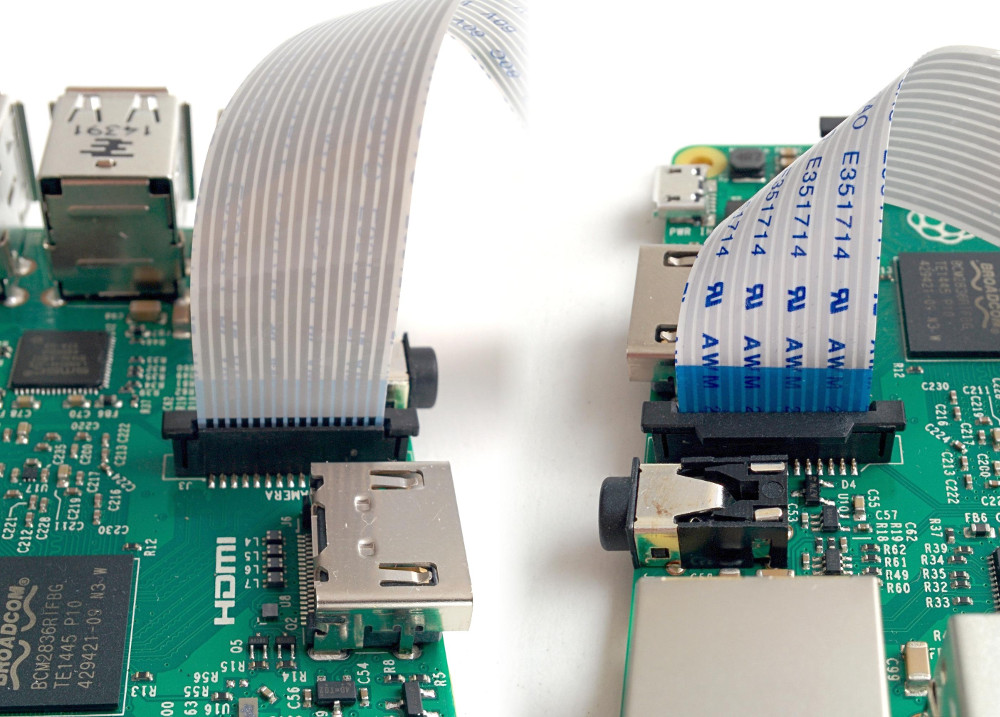
\includegraphics[scale=0.15]{connect-camera.jpg}
    \caption{Conexi\'on de la c\'amara modular}
    \label{fig:ribbon}
\end{figure}

\subsection{Memoria USB}

Tomando en cuenta que se van a capturar fotograf\'ias una vez por hora durante 14 d\'ias se obtiene el n\'umero de im\'agenes que se deben guardar en la memoria USB: $336$. Cada fotograf\'ia tiene una resoluci\'on de \SI{1280x720}{pixels}, cada p\'ixel necesita \SI{3}{B}\footnote{Uno por cada color \emph{RGB}.}, luego cada im\'agen es un archivo de \SI{2764800}{B}.\\

Dicho lo cual, necesitamos una memoria USB de \SI{1}{GB}\footnote{Exactamente \SI{928972800}{B}.}. Hace a\~nos que no se fabrican memorias USB de menos de \SI{4}{GB}; incluso se podr\'ia prescindir de la memoria USB porque el espacio que todav\'ia queda en la memoria mSD es m\'as que suficiente.\\

\subsubsection{3-2-1 backup rule}

Si no se ha cultivado un esp\'iritu aventurero es conveniente tener un \emph{backup}. Seguiremos la conocida regla \textbf{3-2-1} para pol\'iticas de backup (Figura \ref{fig:321bkp}):
\begin{description}
    \item [3] copias de las im\'agenes
    \item [2] copias en medios f\'isicos distintos
    \item [1] copia fuera del lugar f\'isico
\end{description}

Resumiendo, una vez obtenida la imagen se guarda en un directorio de la tarjeta mSD, se hace una copia en la memoria USB y cada \SI{6}{h} se la sube a una carpeta alojada en un servicio cloud.

\begin{figure}
\centering
    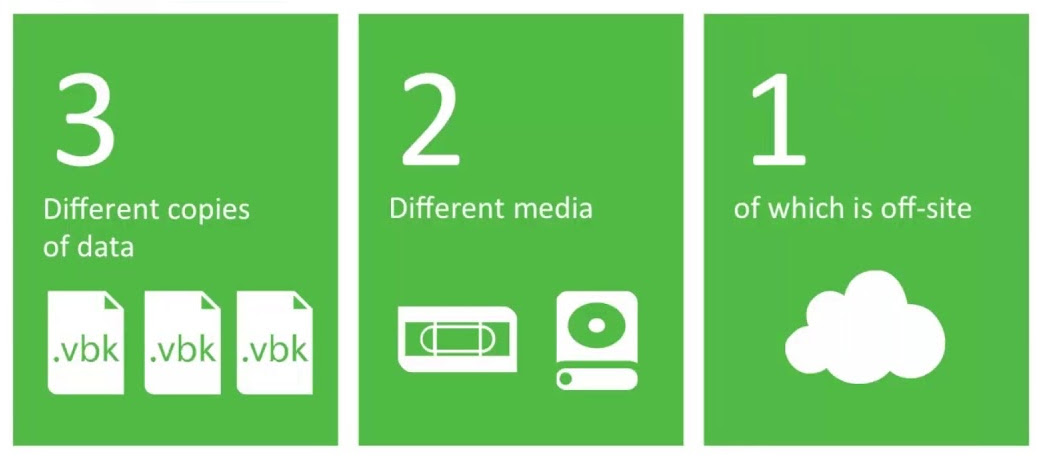
\includegraphics[scale=0.2]{321backup.jpg}
    \caption{3-2-1 backup rule}
    \label{fig:321bkp}
\end{figure}

\subsubsection{Automontaje}

En caso de una grave falla de energ\'ia, al punto de agotar la bater\'ia del power-bank, el sistema va a reiniciar en cuanto la energ\'ia se reestablezca. Se necesita, entonces, automontar la memoria USB. Systemd mediante, esta tarea es crear un archivo \emph{unit} del tipo \emph{mount} en el directorio \texttt{/etc/systemd/system}. Es necesario nombrar esta unit de acuerdo al punto de montaje, en este caso, \texttt{mnt-bkpUSB.mount}.
\begin{lstlisting}
!\#! mkdir /mnt/bkpUSB
!\#! touch /etc/systemd/system/mnt-bkpUSB.mount
\end{lstlisting}

Se busca el UUID\footnote{\emph{Universally Unique IDentifiers}, es una forma un\'ivoca de identificar un dispositivo de almacenamiento.} de la memoria USB:\\
\lstinline{# blkid}\\

Para finalmente editar la unidad de montaje como a continuaci\'on:
\begin{scriptsize}
%\begin{mdframed}
\begin{unitFrame}[/etc/systemd/system/mnt-bkpUSB.mount]
\begin{verbatim}
[Unit]
Description=USB backup
Before=local-fs.target umount.target

[Mount]
What=/dev/disk/by-uuid/87dcbe0c-1e1f-4de7-8f1e-65bcb37a4152
Where=/mnt/bkpUSB
Type=ext4
Options=defaults

[Install]
WantedBy=local-fs.target
\end{verbatim}
\end{unitFrame}
%\end{mdframed}
\end{scriptsize}

Veamos brevemente qu\'e es lo que configuramos en esta \emph{unidad}:

\begin{description}
    \item [Description=] Aqu\'i debe indicarse brevemente y lo m\'as claro que se pueda qu\'e es lo que hace esta unidad.
    \item [Before=] En este caso le estamos indicando a systemd que retrase el inicio de local-fs.target y umount.target hasta que nuestra unidad termine de iniciar. Evitamos as\'i alg\'un conflicto (por ejemplo, que nuestra memoria USB se monte en /media/pi/ y no en /mnt/bkpUSB).\\
    \item [What=] Indicamos unequ\'ivocamente el dispositivo que queremos montar.
    \item [Where=] Indicamos d\'onde queremos montar ese dispositivo.
    \item [Type=] Cu\'al es el sistema de archivos que va a montar (\emph{filesystem}).
    \item [Options=] Las opciones de montaje, que conviene en \'este caso dejarlas predeterminadas.
    \item [WantedBy=] Aqu\'i indicamos qu\'e unidad o servicio va a iniciar a \'esta unidad. No lo maneja systemd directamente, sino cuando se lo instala (cosa que debemos hacer para completar el automontaje, esto es: \lstinline{# systemctl enable mnt-bkpUSB.mount}) se crea un enlace simb\'olico de esta unidad en el directorio \emph{local-fs.target.wants}, que cuando inicia local-fs.target inicia mnt-bkpUSB.mount\footnote{Momento, ?`no le indicamos en \texttt{Before=} que retrase el inicio de local-fs.target?, ?`por qu\'e le decimos ahora que sea local-fs.target quien inicie a mnt-bkpUSB.mount? Brevemente: systemd sabe que tiene que iniciar local-fs.target, no mnt-bkpUSB.mount, a resultas nuestra unidad de automontaje inicia \emph{antes} pero \emph{a pedido} de local-fs.target.}.
\end{description}

Con SysVinit hab\'ia que modificar el archivo \texttt{/etc/fstab} y agregar una l\'inea como la siguiente\footnote{La opci\'on \emph{auto} indica que se automonte.}:
\begin{scriptsize}
\begin{mdframed}
\begin{verbatim}
<file system>       <mount point>   <type>  <options>               <dump>  <pass>
UUID=87dcbe0c-1e1f-4d... /mnt/bkpUSB     ext4    defaults,noatime,auto   0       0
\end{verbatim}
\end{mdframed}
\end{scriptsize}

\subsubsection{Journaling}

No es imprescindible que la memoria USB tenga un sistema de archivos con \emph{journaling}. El journaling es una t\'ecnica implementada en algunos \emph{filesystems} que aseguran la integridad de los archivos; nos permite un alto grado de confianza cuando copiamos archivos de un medio a otro.\\

En los sistemas GNU/Linux es posible elegir entre varios filesystems, donde \textbf{ext4} es el favorito de muchas distribuciones. A efectos de ser prolijos, formateamos la memoria USB con \'ese filesystem\footnote{?`Por qu\'e no ntfs? Porque este informe puede prescindir de \emph{Windows}.}. Desmontamos la memoria USB\footnote{En una rpi2 el primer pendrive es asignado como /dev/sda.} y lo formateamos con una peligrosa facilidad:
\begin{lstlisting}
!\#! umount /dev/sda1
!\#! mkfs.ext4 /dev/sda1
\end{lstlisting}

\section{Servicios}

Los servicios ser\'an expuestos s\'olo en su objetivo, no describiremos el c\'odigo por muy simple que sea. Por ejemplo, vamos a suponer que para tomar una fotograf\'ia s\'olo debe ejecutarse un script al que llamaremos \emph{tomarFoto.sh}\footnote{El script puede estar en cualquier lugar, s\'olo debemos recordar asignarle el permiso de ejecuci\'on.}; para sincronizar\footnote{Sincronizar no es \emph{copiar}, es comparar la carpeta de origen con la de destino y dejarla igual, borrando los archivos que ya no est\'an en la carpeta origen y copiando los que todav\'ia no.} la carpeta de fotograf\'ias en la rpi2 con la carpeta alojada en el servidor \emph{Drive} no necesitamos un script porque se hace con una l\'inea de comando\footnote{Vamos a ignorar el control de errores, porque en alg\'un momento este informe tiene que terminarse.} por lo que la estructura es la misma.\\

Ha llegado el momento de configurar los servicios en systemd. Para entender cabalmente los servicios que se necesitan repasemos los requerimientos.\\

Por cada hora se toma una fotograf\'ia que es guardada en un directorio del sistema, /home/pi/Fotos, y se escribe una entrada registrando el evento. Entonces necesitamos una \emph{unit.timer}: \textbf{tomarFoto.timer}, que active una \emph{unit.service}: \textbf{tomarFoto.service}, que tome la fotograf\'ia y active otra \emph{unit.service}: \textbf{tomarFotoLog.service}, que realice el log. Cada vez que el directorio /home/pi/Fotos cambie (es decir, cuando se crea un nuevo archivo en \'el) se activa una \emph{unit.path}: \textbf{syncUSB.path}, que activa una \emph{unit.service}: \textbf{syncUSB.service} que sincroniza ese directorio con otro directorio en la memoria USB, que a su vez activa una \emph{unit.service}: \textbf{syncUSBLog.service}, que hace un logging\footnote{Acci\'on de realizar un log} de esta acci\'on (Figura \ref{fig:tomarFoto}).\\

\begin{figure}[h!]
\centering
    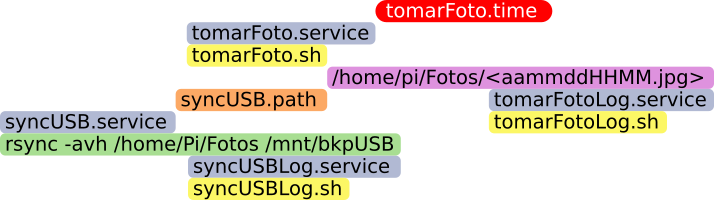
\includegraphics[scale=0.25]{pictos/tomarFoto.png}
    \caption{Algoritmo para tomar una foto}
    \label{fig:tomarFoto}
\end{figure}

Cada \SI{6}{h} se sincroniza la carpeta /home/pi/Fotos con una carpeta en el cloud de Drive y se hace un logging de esta acci\'on. Ya deber\'iamos sospechar lo que necesitamos, una \emph{unit.timer}: \textbf{syncDrive.timer}, que active una \emph{unit.service}: \textbf{syncDrive.service}, que sincronice y que a su vez active una \emph{unit.service}: \textbf{syncDriveLog.service}, que haga el log (Figura \ref{fig:syncDrive}).\\

\begin{figure}[h!]
\centering
    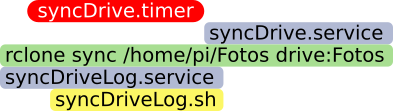
\includegraphics[scale=0.25]{pictos/syncDriver.png}
    \caption{Algoritmo para tomar sincronizar en la nube}
    \label{fig:syncDrive}
\end{figure}

Empecemos por el servicio que justifica este informe: \emph{tomarFoto.service}\\

\begin{lstlisting}
!\#! touch /etc/systemd/system/tomarFoto.service
!\#! chmod 644 /etc/systemd/system/tomarFoto.service!\footnote{Por convenci\'on todos los usuarios tienen permiso de lectura y negados para la ejecuci\'on; y s\'olo el root deber\'ia poder editarlos.}!
!\#! vim /etc/systemd/system/tomarFoto.service
\end{lstlisting}

\begin{scriptsize}
\begin{unitFrame}[/etc/systemd/system/tomarForo.service]
\begin{verbatim}
[Unit]
Description=Captura una foto

[Service]
Type=oneshot
ExecStart=/home/leandro/scripts/tomarFoto.sh
\end{verbatim}
\end{unitFrame}
\end{scriptsize}

Por convenci\'on las unit de servicio se nombran como el servicio que ejecutan.\\

--\emph{Entiendo} ---dice un probable lector---, \emph{?`pero qu\'e es una \emph{unit}?}\\

En el supuesto improbable de que \'ese lector se est\'e anoticiando con \'este informe de systemd, a continuaci\'on una breve descripci\'on. Systemd es el administrador de servicios\footnote{Demonios.} que reemplaza al venerable SysVinit con un enfoque diferente del manejo de recursos, tanto dispositivos, puntos de montaje, sockets, etc. Por ejemplo, el tiempo de booteo se acorta \emph{dram\'aticamente} debido a que systemd implementa una agresiva paralelizaci\'on de los servicios, en contraste con SysVinit que es secuencial. Los scripts y daemons de SysVinit son compatibles con systemd.\\

Una de las ventajas de systemd es su simpleza en la configuraci\'on. La columna vertebral de systemd son las unit: archivos de texto plano que habitan en /lib/systemd/system con una extensi\'on que indica qu\'e tipo de unit es (service, path, mount point, target, timer, device, socket, etc.). Brevemente, una unit describe un recurso y le indica a systemd c\'omo debe activarlo. No todas las unit est\'an activadas al inicio, muchas inician s\'olo cuando son necesarias, optimizando el sistema de manera notable. Cuando una de \'estas units est\'a activa un link simb\'olico se crea en /etc/systemd/system. En este caso de estudio, vamos a crear las unit que se necesitan en este \'ultimo directorio, porque por convenci\'on s\'olo las unit \emph{nativas} del sistema operativo deben estar en /lib/systemd/system.\\

Retomando, la unit tomarFoto.service tiene dos secciones: \emph{[Unit]} y \emph{[Service]}. La primera es opcional (aunque rara vez se omite) y posee informaci\'on de la unit; es com\'un a todas. La otra secci\'on es espec\'ifica de este tipo de unit. 

\begin{description}
    \item [Description=] Esta secci\'on es descriptiva, pensada para la interfase del usuario.
    \item [Type=] Indica c\'omo debe activarse este servicio, \emph{qu\'e tipo de servicio es}. No nos interesa que systemd siga a este servicio luego de ejecutarse, por eso en lugar de \emph{simple} le indicamos \emph{oneshot}.
    \item [ExecStart=] Comandos con sus argumentos que ser\'an ejecutados cuando este servicio inicie. Sin embargo, como le indicamos que el Type es oneshot s\'olo hay que poner uno, que en este caso es tomarFoto.sh que est\'a alojado en el directorio /home/pi/scripts.
\end{description}

Ahora podemos tomar una foto de dos formas\footnote{en el supuesto que el script tomarFoto.sh cumpla lo que promete.}:
\begin{lstlisting}
!\$! /home/pi/scripts/tomarFoto.sh
\end{lstlisting}
o a trav\'es de systemd:
\begin{lstlisting}
!\$! systemctl start tomarFoto.service
\end{lstlisting}

Analicemos la Figura \ref{fig:tomarFoto}, al crear un archivo (la foto) en el directorio /home/pi/Fotos se dispara la unit syncUSB.service, ?`por qu\'e? Por la unit \emph{syncUSB.path}, que le indica a systemd que monitoree ese directorio; y cuando se produce un cambio systemd activa la unit asociada a syncUSB.path: \emph{syncUSB.service}.\\

Entonces, una vez creadas las unit como se hizo con tomarFoto.service procedemos a editarlas:

\begin{scriptsize}
\begin{unitFrame}[/etc/systemd/system/syncUSB.path]
\begin{verbatim}
[Unit]
Description=Monitorea el directorio Fotos

[Path]
PathModified=/home/pi/Fotos
\end{verbatim}
\end{unitFrame}
\end{scriptsize}

Este tipo de unit debe contener una secci\'on \emph{[Path]}

\begin{description}
    \item [PathModified=] Ruta absoluta del directorio o archivo a monitorear.
\end{description}

\begin{scriptsize}
\begin{unitFrame}[/etc/systemd/system/syncUSB.service]
\begin{verbatim}
[Unit]
Description=Sincroniza Fotos con el USB

[Service]
Type=oneshot
ExecStart=rsync -avh /home/pi/Fotos/ /mnt/bkpUSB/
\end{verbatim}
\end{unitFrame}
\end{scriptsize}

En este caso es innecesario crear un script, pues tendr\'ia la misma l\'inea de c\'odigo. El programa \emph{rsync} puede instalarse directamente desde el repositorio de Debian:
\begin{lstlisting}
!\#! aptitude update && aptitude install -y rsync
\end{lstlisting}
\'Esto es, utilizamos el gestor de paquetes \emph{aptitude}\footnote{Se dice que es un poco m\'as expeditivo y eficiente que apt (o apt-get).} para actualizar la base del repositorio y a continuaci\'on instalamos rsync\footnote{Esa continuaci\'on est\'a indicada por los dos signos ampersand (\&\&)}.\\

La estructura de rsync es cl\'asica: comando opciones origen destino

\section{Timers}

Entonces, cada \SI{60}{min} se ejecutan tres scripts:
\begin{enumerate}
    \item tomar foto
    \item sincronizar carpeta de fotos de la rpi2 con la memoria USB
    \item log
\end{enumerate}

Y cada \SI{6}{h} se ejecutan dos scripts:
\begin{enumerate}
    \item sincronizar carpeta de fotos de la rpi2 con el servidor Drive
    \item log
\end{enumerate}

Los servicios son disparados por \emph{systemd}.

\begin{scriptsize}
\begin{mdframed}
\begin{verbatim}
[Unit]
Description=Test del timer de systemd

[Timer]
#OnCalendar=*:0/3
OnCalendar=hourly

[Install]
WantedBy=timers.target
\end{verbatim}
\end{mdframed}
\end{scriptsize}

\section{Conclusi\'on}

La conclusi\'on es que systemd es m\'as complicado pero no nos queda otra.

Para automontar el USB hay que escribir mas cosas que antes, pero no modificamos archivos del sistema.

Systemd parece ir en contra de la filosofia de unix: evitar los programas monoliticos (un programa por cada tarea)

Los manuales estan en: \$ man systemd.{unit, mount, timer}

\end{document}
